\documentclass[a4paper, 12 pt]{article}

\setlength{\voffset}{-0.5cm}


\usepackage[utf8]{inputenc}
\usepackage[T1]{fontenc}
\usepackage[german]{babel}

\usepackage{graphicx}
\usepackage[absolute]{textpos}

\usepackage{amsmath}
\usepackage{hyperref}
\usepackage[nameinlink]{cleveref}
\crefname{figure}{Abb.}{Abb.}

\usepackage{pflichtenheft}

%für Glossar
\usepackage[nonumberlist, section]{glossaries}

%Glossareinträge
\makenoidxglossaries

	\newglossaryentry{IoT}{
		name={Internet der Dinge},description={Das Internet der Dinge (englisch: Internet of Things, IoT) ist ein Begriff dafür, dass in der modernen Welt, physische und virtuelle Gegenstände miteinander über das Internet verbunden sind und dadurch zusammenarbeiten können.}
	}

	\newglossaryentry{ogc}{
		name={OGC},description={Das \textbf{O}pen \textbf{G}eospatial \textbf{C}onsortium ist eine gemeinnützige Organisation, die gegründet wurde, um frei benutzbare, allgemeingültige Standards für die raumbezogene Informationsverarbeitung (insbesondere Geodaten) festzulegen. \\
		http://www.opengeospatial.org/}
	}

	\newglossaryentry{stApi}{
		name={SensorThings API},description={Allgemeiner einheitlicher Standard um Verbindung zwischen Sensoren, deren Ort und Umgebung und den von ihnen erzeugten Daten herzustellen. Link zur genauen Beschreibung: \\
		http://developers.sensorup.com/docs/}
	}

	\newglossaryentry{frost}{
		name={FROST-Server},description={Der \textbf{FR}aunhofer \textbf{O}penSource \textbf{S}ensor\textbf{T}hings-Server ist die erste komplette quelloffene Implementierung der \gls{ogc} \gls{stApi}. \\
		https://www.iosb.fraunhofer.de/servlet/is/80113/ \\
		https://github.com/FraunhoferIOSB/FROST-Server}
	}

	\newglossaryentry{csvExcel}{
		name={CSV-/Excel-Datei},description={CSV (Comma Seperated Value, .csv) und Excel (.xlsx/.xls) sind gängige Dateiformate zum Speichern von Daten (hier speziell: Sensor-Daten) in Tabellenform}
	}

	\newglossaryentry{int}{
		name={Integer},description={Integer (deutsch: Ganzzahl) ist ein Datentyp zum speichern ganzzahlige Werte}
	}

	\newglossaryentry{magicnum}{
		name={Magic Number},plural={Magic Numbers},description={Deutsch: Magische Zahl. Ein im Quellcode eines Programms auftauchender Zahlenwert, dessen Bedeutung sich nicht unmittelbar erkennen lässt}
	}

	\newglossaryentry{aggr}{
		name={Aggregation},plural={Aggregationen},description={Eine Aggregation beschreibt eine Operation auf einem Datensatz, die die Daten zusammenfasst. Dazu gehören zum Beispiel das Bilden der Summe, des Durchschnitts oder des Minimums bzw. Maximums}
	}

	\newglossaryentry{jre}{
		name={JRE},description={Mit der Java-Laufzeitumgebung (\textbf{J}ava \textbf{R}untime \textbf{E}nvironment) werden Programme (Java-Anwendungen) weitgehend unabhängig vom darunter liegenden Betriebssystem ausgeführt}
	}

	\newglossaryentry{headless}{
		name={headless},description={Als headless (kopflos) bezeichnet man Server/Computer die über keine grafische Ausgabe, also keinen Bildschirm oder verfügen. Diese Systeme haben als Steuerungsmöglichkeit in vielen Fällen eine Netzwerkverbindung}
	}

	\newglossaryentry{js}{
		name={JavaScript},description={JavaScript ist eine Programmiersprache, die hauptsächlich auf Webbrowsern Anwendung findet}
	}

	\newglossaryentry{logdat}{
		name={Log-Datei},description={Eine Log-Datei, auch Protokoll-Datei, speichert automatisch Protokollinformationen über bestimmte Aktionen von Anwendungen auf einem Computersystem}
	}

	\newglossaryentry{docker}{
		name={Docker},description={Docker ist eine Software zur Isolierung von Anwendungen. Docker vereinfacht die Bereitstellung von Anwendungen, weil sich sogenannte Container, die alle nötigen Pakete enthalten, leicht als Dateien transportieren und installieren lassen. Website: \\
		https://www.docker.com/}
	}

	\newglossaryentry{ssl}{
		name={SSL},description={SSL steht für \textbf{S}ecure \textbf{S}ockets \textbf{L}ayer und ist die Standardtechnologie für die Absicherung von Internetverbindungen und den Schutz sensibler Daten, die zwischen zwei Systemen übertragen werden}
	}

	\newglossaryentry{https}{
		name={HTTPS},description={\textbf{H}yper\textbf{T}ext \textbf{T}ransfer \textbf{P}rotocol \textbf{S}ecure (HTTPS) ist ein sicheres Hypertext-Übertragungsprotokoll, das \gls{ssl} benutzt}
	}

	\newglossaryentry{regex}{
		name={RegEx},description={\textbf{Reg}ular \textbf{Ex}pressions (Regex, regulärer Ausdrucke) dienen der Beschreibung von Zeichenketten mit ähnlichem Format. Sie können als Filterkriterien in der Textsuche benutzt werden. Dabei wird der Text mit dem Muster des regulären Ausdrucks (RegEx) verglichen.}
	}

	\newglossaryentry{iosb}{
		name={Fraunhofer IOSB},description={Das Fraunhofer-Institut für Optronik, Systemtechnik und Bildauswertung ist in der angewandten Forschung und Entwicklung im Fach Ingenieurwissenschaften auf dem Gebiet der Informations- und Kommunikationstechnologie aktiv. So entwickelten sie unter anderem den \gls{frost}, der für dieses Projekt von zentraler Bedeutung ist. Website: \\
		https://www.iosb.fraunhofer.de/ }
	}

	\newglossaryentry{thing}{
		name={Thing},plural={Things},description={Ein Thing (deutsch: Gegenstand/Ding) ist nach Definition der \gls{stApi} ein Objekt der physischen oder virtuellen Welt. Es benötigt einen Namen und eine Beschreibung. Es können sich ein oder mehrere \glspl{ds} auf ein Thing beziehen}
	}

	\newglossaryentry{ds}{
		name={Datastream},plural={Datastreams},description={Ein Datastream ist eine fortlaufende Sammlung von Messungen (\glspl{obs}) des selben \gls{sensor}s und der selben \gls{obsprop}. Multi-Datastreams haben mehrere \glspl{obsprop}}
	}
	
	\newglossaryentry{obsprop}{
		name={ObservedProperty},plural={ObservedProperties},description={Eine ObservedProperty (deutsch: beobachtete Eigenschaft) spezifiziert das Phänomen einer Beobachtung (\gls{obs})}
	}

	\newglossaryentry{location}{
		name={Location},plural={Locations},description={Beschreibt den Ort eines oder mehrerer \glspl{thing}}
	}

	\newglossaryentry{obs}{
		name={Observation},plural={Observations},description={Eine Observation (deutsch: Beobachtung) ist die Aktion des Messens eines Wertes einer Eigenschaft}
	}

	\newglossaryentry{sensor}{
		name={Sensor},description={Ein Sensor misst eine Eigenschaft um eine Approximation des Wertes der Eigenschaft zurückzugeben}
	}

	

	

\author{Adrian Cierpka \and  Maximilian Göckel  \and Frithjof Marquardt \and Fabian Nguyen \and Andreas Wieland}
\title{CHILLImport: Weboberfläche zum Management von Sensordaten\\Pflichtenheft}


\hyphenation{Ü-ber-tra-gungs-fort-schrit-te}

\begin{document}

\maketitle
\newpage
\tableofcontents
\newpage

	%TODO
	\section{Produktübersicht}

	%Max
	Eines der wichtigsten Themen im \gls{IoT} (IoT) sind Sensordaten. Mit ihnen lassen sich Informationen über die Dinge um uns herum herausfinden. Sensordaten werden schon seit Jahren aufgenommen, gesammelt und verarbeitet. Ein Ziel des IoT ist es, mit mehr Sensoren mehr Daten aufzunehmen. \\

	Damit diese Massen von Messwerten und Metadaten eines Sensors in ihrer eigenen Vielfalt effizient verarbeitet werden können, bedarf es einem einheitlichen Standard. Das \gls{ogc} stellt als Standardisierungsgremium dazu die \gls{stApi} \footnote{http://docs.opengeospatial.org/is/15-078r6/15-078r6.html} bereit, welche die durch jahrelange Erfahrung im Arbeiten mit Sensordaten entstandenen Konzepte an die Anforderungen und Möglichkeiten neuer Schnittstellen anpasst. \\

	Der \textbf{FR}aunhofer\textbf{O}penSource\textbf{S}ensor\textbf{T}ings-Server (\gls{frost})\footnote{https://www.iosb.fraunhofer.de/servlet/is/80113/} des \gls{iosb} ist eine Implementierung des SensorThings-Standards. Der Server will die \gls{stApi} ressourcenschonend und mit hoher Leistungsfähigkeit bereitstellen. Das Institut hat sich direkt von Anfang an dazu entschlossen, die Software erreichbarer zu machen und entwickelte den Server als Open Source Software\footnote{https://github.com/FraunhoferIOSB/FROST-Server}. \\

	Neben dem \gls{frost} stellt das \gls{iosb} auch den FROST-Client bereit, eine Bibliothek, die hilft, auf die \gls{stApi} zuzugreifen\footnote{https://github.com/FraunhoferIOSB/FROST-Client}. \\
	\ \\
	Die hier entwickelte Software CHILLImport stellt zu dem \gls{frost} eine Webseite bereit, die es Nutzern ermöglicht, Daten aus Tabellen (beispielsweise einer Excel-Tabelle) in ein \gls{stApi}-freundliches Format zu konvertieren und auf eine \gls{frost}-Instanz hochzuladen. Die Software soll auf der einen Seite so einfach zu bedienen sein, dass auch technisch unerfahrene Nutzer die Grundfunktionen nutzen können. Auf der anderen Seite soll sie stark konfigurierbar sein, um auch erfahrene Nutzer mit hohen Ansprüchen zufrieden zu stellen.\\

\newpage
	\section{SensorThings API}

	Die \gls{stApi} besteht aus folgenden Entitäten, die miteinander im Zusammenhang stehen. Jede Entität hat bestimmte Eigenschaften. Diese und die Beziehungen sind im unten abgebildeten UML-Diagramm\footnote{http://docs.opengeospatial.org/is/15-078r6/15-078r6.html} (\cref{fig:ogc}) dargestellt. \\
	\begin{enumerate}
	
	\item Thing (Gegenstand): Ein Objekt aus der realen Welt (physisches Thing) oder ein virtuelles Thing
	\item Locations (Orte): Beschreiben den Ort eines oder mehrerer Things
	\item HistoricalLocations (historische Orte): Beschreiben die zuletzt bekannten und vergangenen Orte des/der Things zusammen mit ihrem Zeitpunkt
	\item Sensor: Misst eine Eigenschaft um eine Approximation des Wertes der Eigenschaft zurückzugeben
	\item Observation (Beobachtung): Die Aktion des Messens eines Wertes einer Eigenschaft
	\item ObservedProperty (beobachtete Eigenschaft): Spezifiziert das Phänomen einer Beobachtung
	\item FeatureOfInterest: Eine Beobachtung erzeugt einen Wert, welcher an ein Phänomen gekoppelt ist. Dieses Phänomen ist Teil eines Features, welches das FeatureOfInterest einer Beobachtung ist
	\item Datastream (Datenfluss): Eine Menge von Beobachtungen über die selbe ObservedProperty vom selben Sensor   
	\end{enumerate}
	Die genaue Beschreibung aller Elemente und Beziehungen sind zu finden unter: \\
	\href{http://developers.sensorup.com/docs/}{SensorUp Developer Page}\footnote{http://developers.sensorup.com/docs/}\\
	\href{https://en.wikipedia.org/wiki/SensorThings_API}{Wikipedia-Artikel zur API}\footnote{https://en.wikipedia.org/wiki/SensorThings\_API}\\
	\href{http://docs.opengeospatial.org/is/15-078r6/15-078r6.html}{OGC-Dokumentation von SensorThings}\footnote{http://docs.opengeospatial.org/is/15-078r6/15-078r6.html}\\

\begin{figure}
\centering
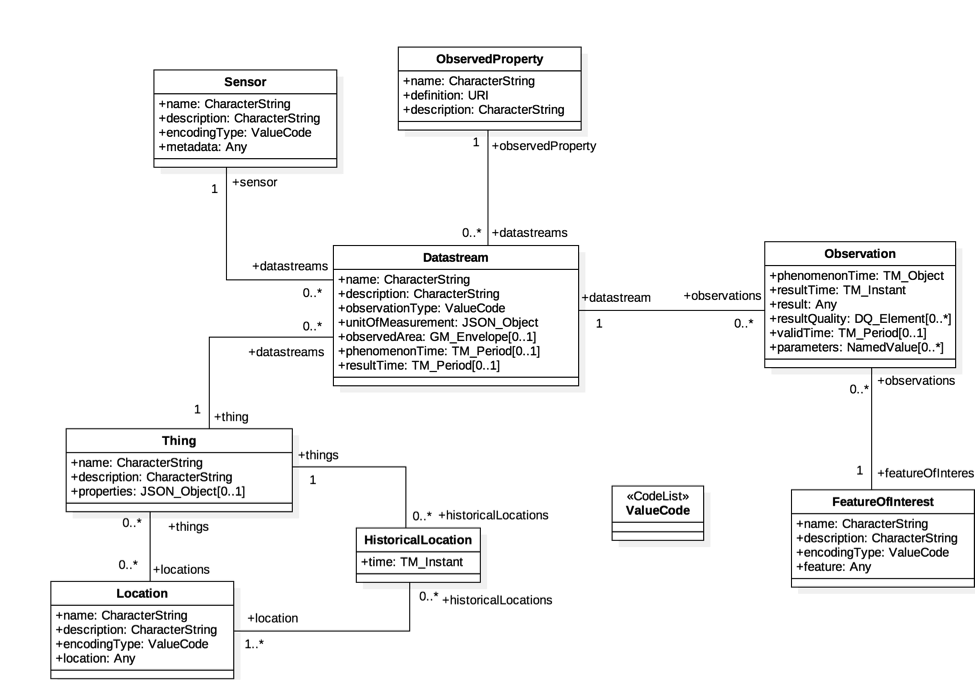
\includegraphics[scale=0.8]{images/ogc}
\caption{\label{fig:ogc}Klassendiagramm der SensorThings API}
\end{figure}

\newpage
\section{Zielbestimmung}
	\subsection{Musskriterien}
	
	
	\criterium{Import von Messwerten}{crt:data}
	Die Sensor-Messwerte sollen aus Tabellen im \gls{csvExcel}format importiert werden.

	\criterium{Konvertierung des Formats der Sensordaten}{crt:conv}
	Die Daten sollen aus den beliebigen Datenformaten und Anordnungen innerhalb der Quelldatei in den einheitlichen Standard der \gls{stApi} konvertiert werden.
    Damit entsprechen sie dem Standard der Daten auf einem \gls{frost}.
	
	\criterium{Erstellen, Abspeichern und Laden von Konfigurationen}{crt:conf}
	Der Benutzer soll Spaltenformat, Datenformat und insbesondere das Datums- und Zeitformat einstellen und als Konfiguration abspeichern können.
    Diese Konfigurationen sollen später auch wieder geladen werden können.

	\criterium{Datentyptransformationen}{crt:trf}
	Alle Werte sind in der Quelldatei als String vorhanden und müssen, bevor sie auf den \gls{frost} geladen werden, in den passenden Datentyp (bspw. \gls{int}) umgewandelt werden.
	Sonderwerte (\glspl{magicnum}) sollen nicht auf den \gls{frost} geladen, sondern separat behandelt werden.	
	
	\subsection{Wunschkriterien}
	
	
	\criteriumOptional{Standard-Konfiguration}{crt:std}
	Für eine Auswahl gängiger Eingabedateien wird dem Benutzer eine Liste vordefinierter Konfigurationen, bestehend aus Spaltenformat, Datenformat und Datums- und Zeitformat, vorgeschlagen.
	\criteriumOptional{Überprüfung auf Duplikate}{crt:dupl}
	Beim Upload der Daten auf den \gls{frost} werden diese mit den bestehenden Daten abgeglichen und Duplikate werden nicht erneut gespeichert.
	\criteriumOptional{Rückgabe nicht bearbeiteter Datensätze in neuer \gls{csvExcel}}{crt:ruck}
	Bei (teilweise) fehlgeschlagener Übertragung zum \gls{frost} werden die nicht übertragenen Daten in einer \gls{csvExcel} an den Benutzer zurückgegeben.
	\criteriumOptional{Korrektur fehlerhafter Daten}{crt:korr}
	Dem Benutzer wird es ermöglicht automatisch erkannte fehlerhafte Datensätze in der Weboberfläche zu korrigieren.
	\criteriumOptional{Import von Fremdquellen wie anderen Webseiten}{crt:web}
	Es soll möglich sein, als Quelldatei auch einen entfernten Speicherort, zum Beispiel einen Weblink, anzugeben.
	\criteriumOptional{Automatisierte Daten-Aktualisierung}{crt:akt}
	Bei Import von Daten von einer entfernten Adresse wird eine automatische, regelmäßige Übertragung angeboten.
	\criteriumOptional{Import kompletter Datensätze von anderem \gls{frost}}{crt:frost}
	Der Benutzer hat zusätzlich die Möglichkeit, Daten von einem anderen \gls{frost} zu kopieren.
	\criteriumOptional{Komplexe Transformationen/\gls{aggr}}{crt:aggr}
	\gls{aggr} auf ausgewählten Daten (bspw. Summe oder Durschnitt) werden dem Benutzer bereitgestellt.
	\criteriumOptional{Automatische Formaterkennung}{crt:form}
    Aus der Quelldatei werden Spaltenformat, Datenformat und Datums- und Zeitformat automatisch erkannt und dem Benutzer eine passende Konfiguration vorgeschlagen.
	\criteriumOptional{Automatische Sprachauswahl}{crt:lang}
	Die Anwendung übernimmt automatisch die in Browser eingestellte Sprache.
	

	\subsection{Abgrenzungskriterien}
	
	\criteriumNot{Keine Bearbeitung vorhandener Daten}{crt:no-edit}
Die Bearbeitung (ändern, löschen) bereits vorhandener Daten auf einem \gls{frost} wird nicht unterstützt.
	\criteriumNot{Keine Benutzerverwaltung}{crt:no-user}
Es wird keine Benutzerverwaltung mit verschiedenen Benutzerkonten bereitgestellt. Authentifizierung wird ebenfalls nicht unterstützt.
Jeder Benutzer kann somit die gespeicherten Konfigurationen aller Benutzer sehen und verwenden.
	\criteriumNot{Keine mobilen Endgeräte}{crt:no-mobile}
	Die Software muss nicht auf mobilen Endgeräten laufen können.

\pagebreak
\section{Produkteinsatz}
\subsection{Anwendungsbereiche}
Die Software kommt überall dort zum Einsatz, wo Sensordaten gesammelt werden, aber nicht automatisch in den FROST-Server übertragen werden können.\\
Als Beispiel ist ein Forschungsprojekt zu nennen, bei dem die Sensordaten in Tabellenform vorliegen. Diese Daten sollen in eine FROST-Instanz hochgeladen und ggf. weiterverarbeitet werden. Ebenso können neue Sensordaten durch den Mitarbeiter einer Firma (z.B. Stadtwerke) importiert werden.\\
Die Integration bestehender Sensordaten in Tabellenform stellt auch einen großen Anwedungsbereich dar.
	

	\subsection{Zielgruppen}
	Die Software ist auf zwei Zielgruppen ausgelegt.\\
	\begin{enumerate}
		\item Personen, welche einfach Sensordaten auf einen FROST-Server laden möchten, ohne die Konfigurationen zu ändern
		
		\begin{itemize}
			\item Wenig bis keine technischen Kenntnisse
			\item Fokus auf einfache und schnelle Bedienung der Software
		\end{itemize}
		
		\item Nutzergruppe, die ihre eigenen Konfigurationen erstellt
		\begin{itemize}
			\item Umfangreiches Wissen im Umgang mit der Software
			\item Fokus auf komplexe Einstellungsmöglichkeiten in den Konfigurationen
		\end{itemize} 
	\end{enumerate}
	
\subsection{Betriebsbedingungen}
\begin{itemize}
	\item Es wird vorausgesetzt, dass ausreichend Speicherplatz auf dem Server verfügbar ist
	\item Die Software soll ununterbrochen laufen, d.h. die Produktumgebung muss sicherstellen, dass es nicht zu Störungen (Unterbrechung der Stromversorgung, plötzliches herunterfahren o.ä.) kommt
	\item Da Uploads teilweise sehr lange dauern können und der Nutzer nicht immer zwingend anwesend ist, muss die Software problemfrei unüberwacht laufen können
\end{itemize}
	
\section{Produktumgebung}
Die Produktumgebung teilt sich auf in den Webserver, auf dem das Produkt läuft, und den Client, den der Nutzer nutzt um die Webseite aufzurufen. Für beide sind die Umgebungen stark unterschiedlich:
Server:
\begin{itemize}
	\item Unix/Linux
	\item Java \gls{jre}
	\item Kleiner Webserver
	\begin{itemize}
		\item \gls{headless}
		\item Unicore CPU
		\item 1-2GB RAM
		\item Speichermedium mit genug Speicherplatz für Software und temporäre Daten (8GB stark ausreichend)
	\end{itemize}
	\item Konnektivität mit dem \gls{frost}
	\item Erreichbarkeit durch Nutzer-Client
\end{itemize}

\noindent Client:

\begin{itemize}
	\item Moderner Desktop-Webbrowser
	\item Aktiviertes \gls{js}
	\item Netzwerkanschluss an den Web-Server
\end{itemize}


\section{Seitenentwürfe}

\subsection{Hauptseite}
Die Software stellt eine Weboberfläche zum Einfügen von Sensor-Datensätzen auf einen \gls{frost} zur Verfügung. 
Dieser Zielserver wird einmalig beim erstmaligen Aufsetzen der Software eingestellt und ist nicht über das Webinterface einstellbar. 
Ein Entwurf für die Hauptseite der Weboberfläche ist in \cref{fig:guiMain} (siehe Anhang \cref{fig:guiMainA} für vergrößerte Darstellung) zu sehen.
\\

\begin{figure}[htbp]
\centering
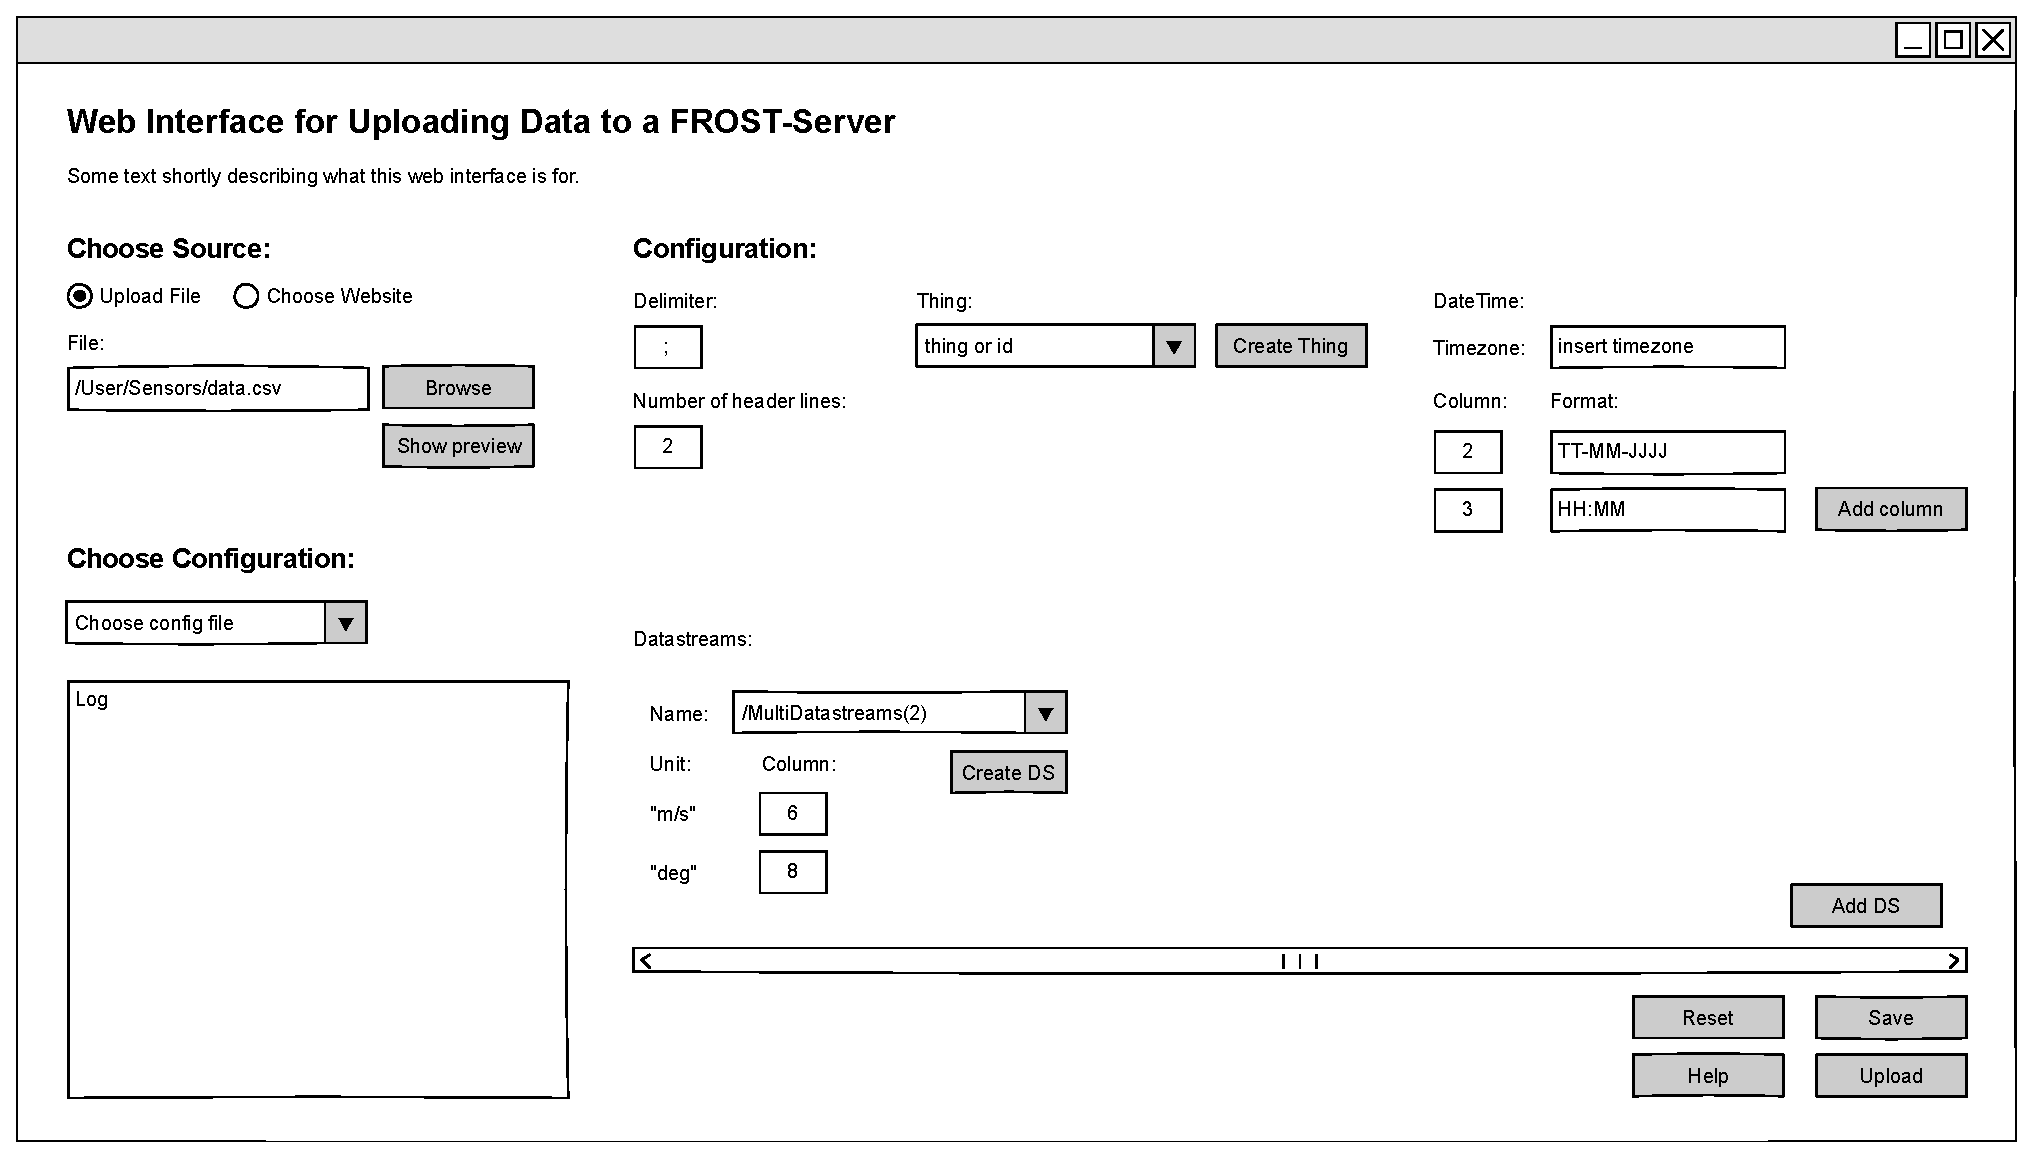
\includegraphics[scale=0.4]{images/gui}
\caption{\label{fig:guiMain}Hauptseite der Weboberfläche}
\end{figure}
Beim Aufrufen der Weboberfläche ist zu Beginn nur der Bereich zum Auswählen der Quelldatei sichtbar. 
Nach dem Einstellen der Quelle wird das Dateiformat überprüft und ein passender Konfigurator (für das Spaltenformat der Datei und das Format der Daten in den Spalten) wird sichtbar. \\

Über das Log werden eventuelle Fehlermeldungen und Übertragungsfortschritte angezeigt. Unter \string"Choose Configuration\string" lässt sich eine auf dem Server gespeicherte Konfigurationsdatei auswählen. Dort bieten sich folgende Möglichkeiten:
\begin{itemize}
\item Unter "{Configuration}" kann eingestellt werden, in welcher Form die Daten in der Quelldatei angespeichert sind, um diese dann in den vom \gls{frost} verwendeten \gls{ogc}-Standard zu konvertieren.
\item Zuerst ist das Trennsymbol für die Spalten in der Quelldatei und die Anzahl der Kopfzeilen (nicht zum Datensatz gehörige Zeilen) anzugeben. 
\item Dann kann das zu den Daten gehörige \gls{thing} von schon auf dem \gls{frost} existierenden \glspl{thing} ausgewählt werden. Falls es benötigt wird, lässt sich über den "{Create Thing}"{-Button} ein neues \gls{thing} erstellen. (siehe \cref{fig:thing})
\item Unter "{DateTime}"{ ist} das Datumsfomat einstellbar. Erst wird die Zeitzone eingegeben und danach lassen sich das Format für das Datum bzw. die Zeit als \gls{regex} und die zugehörige Spaltennummer angeben.
\item Abschließend lassen sich ein oder mehrere (Multi-)\glspl{ds} auswählen. Existiert der (Multi-)\gls{ds} noch nicht, kann er über "{Create DS}"{ erstellt} werden. Mit Hilfe des "{Add DS}"{-Buttons} lassen sich weitere (Multi-)\glspl{ds} hinzufügen. Anschließend lassen sich wieder die zu den Daten gehörigen Spalten in der Quelldatei einstellen.
\item Außerdem bietet die Weboberfläche über den "{Save}"{-Button} die Möglichkeit, eine bestehende Konfiguration auf dem Server abzuspeichern bzw. über den "{Reset}"{-Button} auf die Standard-Konfiguration zurückzusetzen.
\item Über den "{Upload}"{-Button} werden die Daten auf den \gls{frost} hochgeladen.
\item Der "{Help}"{-Button} ermöglicht den Zugriff auf eine Kurzanleitung für das Webinterface.
\end{itemize}

\subsection{Thing erstellen}
Wie in \cref{fig:thing} dargestellt, müssen Name, Beschreibung und Eigenschaften gewählt werden, um ein \gls{thing} zu erstellen. Über den "{Add property}"{-Button} kann eine weitere Eigenschaft als Key-Value-Paar hinzugefügt werden. Abschließend muss eine bestehende \gls{location} gewählt bzw. eine neue erstellt werden (siehe \cref{fig:loc}).

\begin{figure}[htbp]
\centering
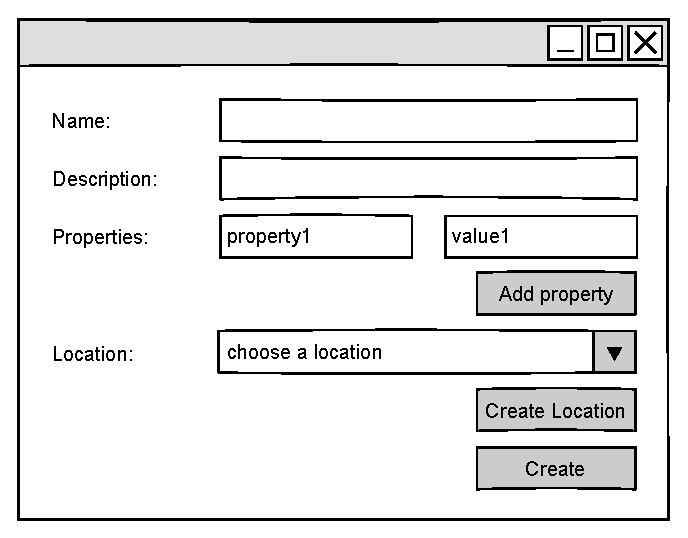
\includegraphics[scale=0.8]{images/thing}
\caption{\label{fig:thing}Dialogfenster zum Erstellen eines Things.}
\end{figure}


\subsection{Datastream erstellen}
\cref{fig:ds} zeigt das Dialogfenster zum Erstellen eines (Multi-)Datastreams. 
\begin{figure}[htbp]
\centering
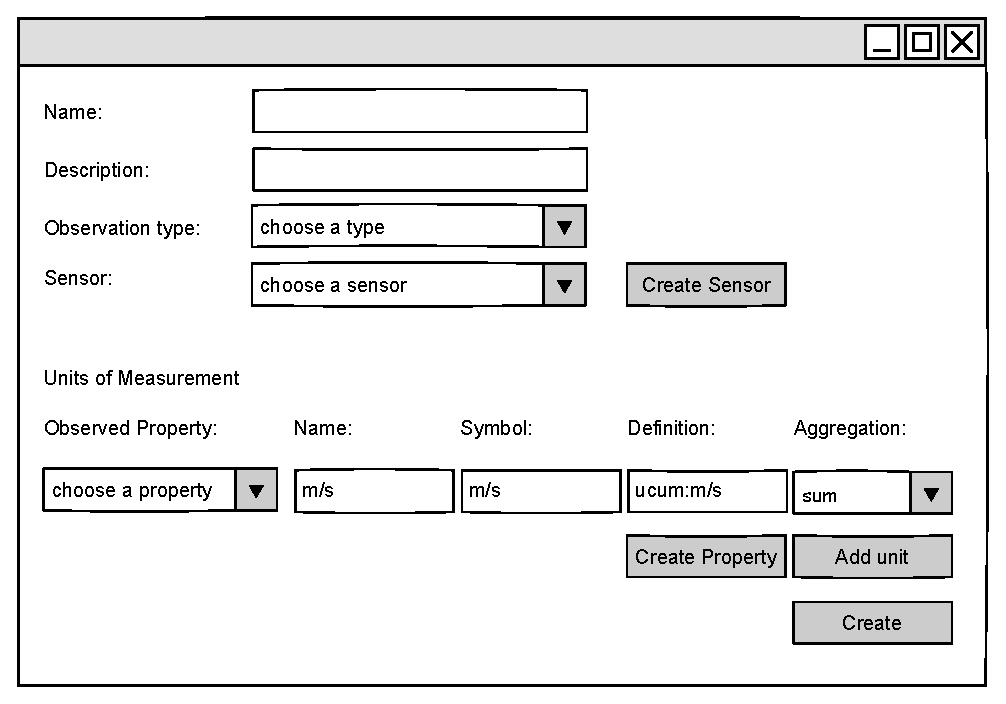
\includegraphics[scale=0.8]{images/datastream}
\caption{\label{fig:ds}Dialogfenster zum Erstellen eines Datastreams.}
\end{figure}
Es müssen erst Name, Beschreibung, Observation Type und ein \gls{sensor} gewählt werden. Soll dafür ein neuer \gls{sensor} angelegt werden, existiert der "{Create Sensor}"{-Button} (siehe \cref{fig:sensor}).\\

Im unteren Teil lassen sich die zugehörigen Einheiten für eine Messwertreihe festlegen. Existiert eine solche Einheit noch nicht, lässt sie sich über den "{Create Property}"{-Button} anlegen (siehe \cref{fig:oprop}). Unter \string"Aggregation\string" lässt sich auswählen, ob alle Daten importiert werden sollen, oder nur eine Aggregation dieses Datensatzes. Mit dem "{Add unit}"{-Button} kann eine weitere Messwertreihe hinzugefügt werden. Hat ein \gls{ds} mehr als eine solche Größe, wird er als Multi-\gls{ds} verwaltet.



\subsection{Sensor, ObservedProperty oder Location erstellen}
Das Erstellen eines \gls{sensor}s (siehe \cref{fig:sensor}), einer \gls{obsprop} (siehe \cref{fig:oprop}) oder einer \gls{location} (siehe \cref{fig:loc}) verläuft, indem alle Textfelder des jeweiligen Dialogfeldes passend ausgefüllt werden und anschließend der "{Create}"{-Button} gedrückt wird.

\begin{figure}[htbp]
\centering
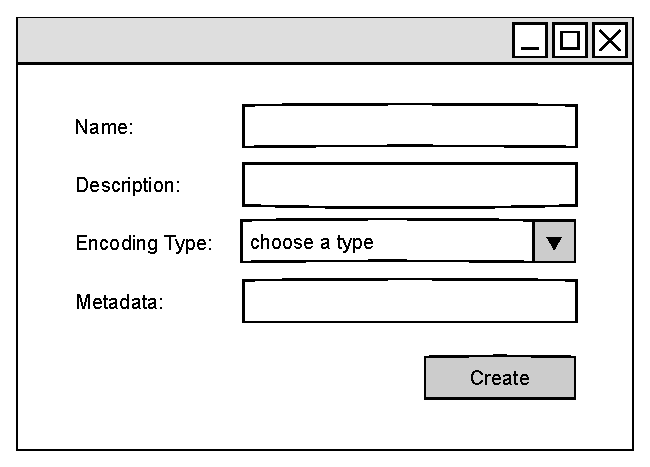
\includegraphics[scale=1]{images/sensor}
\caption{\label{fig:sensor}Dialogfenster zum Erstellen eines Sensors.}
\end{figure}

\begin{figure}[htbp]
\centering
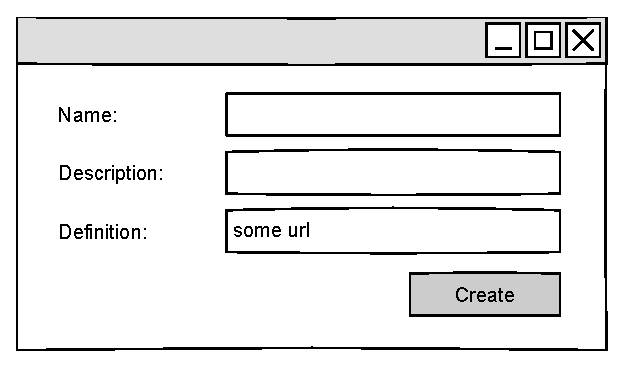
\includegraphics[scale=1]{images/oprop}
\caption{\label{fig:oprop}Dialogfenster zum Erstellen eines Things.}
\end{figure}

\begin{figure}[htbp]
\centering
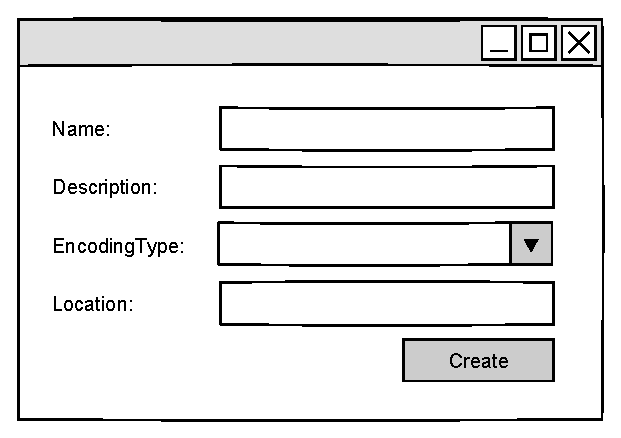
\includegraphics[scale=1]{images/loc}
\caption{\label{fig:loc}Dialogfenster zum Erstellen einer Location.}
\end{figure}

\newpage
\section{Funktionale Anforderungen}
\subsection{Erforderliche funktionale Anforderungen}
	
	\functionality{Auswahlmöglichkeit der Datenquelle}{fnc:quelle}
	\fulfills{crt:data}
	\fulfills{crt:web}
	\fulfills{crt:frost}
	Die Datenquelle ist frei wählbar aus den folgenden Möglichkeiten:
		\begin{itemize}
			\item eine Datei
			\item externe Webseite
			\item externer Server (optional)
		\end{itemize}
		
	\functionality{Laden und speichern von Konfigurationen}{fnc:loadsave}
	\fulfills{crt:conf}
	
	\functionality{Erstellen von Konfigurationen}{fnc:create}
	\fulfills{crt:conf}
	Beim Erstellen einer Konfiguration für das Formatieren der Daten aus der Quelldatei ist folgendes einstellbar:
	\begin{itemize}
			\item Spaltenseperator
			\item Anzahl der Kopfzeilen
			\item Einstellen der Datumsspalte/n
			\item Format des Datums
			\item Auswählen und Erstellen von
			\begin{itemize}
				\item \glspl{thing}
				\item \glspl{location}, für neue \glspl{thing}
				\item \glspl{ds}
				\item \gls{sensor}s, für neue \glspl{ds}
				\item \glspl{obsprop}, für neue \glspl{ds}
			\end{itemize}
			\item Spaltenauswahl für Datenextraktion
		\end{itemize}
	
	\functionality{Auswahlmöglichkeit des Zielservers}{fnc:target}
	\fulfills{crt:data}
	Der Zielserver wird einmalig beim Aufsetzen der Software gewählt und ist danach nur noch durch das Ändern der Konfigurationsdatei zu bearbeiten.
	
	\functionality{Hochladen der Daten auf den \gls{frost}}{fnc:upload}
	\fulfills{crt:data}
	
	\functionality{Formatieren der Daten in \gls{ogc} \gls{stApi} Standard}{fnc:conv}
	\fulfills{crt:conv}
	\fulfills{crt:trf}
	Vor dem Hochladen der Daten aus der Quelldatei werden diese aus ihrem Format (als String gespeichert) in andere passende Datentypen transformiert und auf den \gls{ogc} \gls{stApi} Standard gebracht.
	
	\functionality{Fehlermeldungen}{fnc:fehler}
	\fulfills{crt:korr}
	Für folgende Fehler sollen Fehlermeldungen erscheinen:
	\begin{itemize}
			\item Fehler in Datenzeilen
			\item Verbindungsfehler zum \gls{frost}
			\item Fehlerhafte Quelldatei
		\end{itemize}
	
	\functionality{Anlegen einer \gls{logdat}}{fnc:log}
	Um Fehler einfacher zu reproduzieren und beheben, wird eine Log-Datei angelegt, die folgendes speichert:
	\begin{itemize}
			\item Historie von Uploads
			\item Fehlermeldungen
		\end{itemize}
	

	\subsection{Gewünschte funktionale Anforderungen}
	
	
	\functionality{Bereitstellen einer Default-Konfiguration}{fnc:default}
	\fulfills{crt:std}
	
	
	\functionality{Duplikaterkennung}{fnc:dupl}
	\fulfills{crt:dupl}
	Bevor Daten hochgeladen werden, werden diese mit den Daten im \gls{frost} abgeglichen, um das Hochladen redundanter Daten zu vermeiden.
	
	\functionality{Fehlerkorrektur}{fnc:korr}
	\fulfills{crt:korr}
	Werden beim Formatieren der Daten Fehler festgestellt, wird dem Nutzer die Möglichkeit gegeben, die Daten zu korrigieren bzw. seine Konfiguration anzupassen.	
	
	\functionality{Rückgabe von Fehlerhaften Zeilen in einer neuen \gls{csvExcel}}{fnc:ruck}
	\fulfills{crt:ruck}
	Beim Upload nicht bearbeitete Zeilen aus der Quelldatei werden in eine Datei geschrieben und dem Nutzer zur Verfügung gestellt.
	
	\functionality{Auswahlmöglichkeit komplexer \gls{aggr} auf Daten}{fnc:aggr}
	\fulfills{crt:aggr}
	Der Nutzer kann aus folgenden Aggregationen für seine Datensätze wählen:
	\begin{itemize}
			\item Summe
			\item Minimum
			\item Maximum
			\item Durchschnitt
	\end{itemize}
	Diese Operationen sind nur spaltenweise möglich (d.h. nur auf der Messreihe für einzelne Größen).
	
	\functionality{Regelmäßige Daten-Aktualisierung}{fnc:akt}
	\fulfills{crt:akt}
	Quelldateien von externen Webseiten können regelmäßig ohne erneute Aktion vom Nutzer abgerufen und verarbeitet werden.
	
	\functionality{Formaterkennung}{fnc:form}
	\fulfills{crt:form}
	Beim Hochladen einer Datei wird diese direkt analysiert und ein Spalten-, Daten- und Datumsformat vorgeschlagen, um das Einstellen der Konfiguration zu erleichtern.
	
	
	\functionality{Kurzanleitung auf der Weboberfläche}{fnc:help}
	
	
	
	%TODO Nummerierung der Wunschkriterien in Fließtext
	\section{Produktdaten}
	
	Bei den Daten, die auf dem Server gespeichert werden müssen, wird unterschieden zwischen Nutzerdaten und Systemdaten.
	
\begin{itemize}
	\item Nutzerdaten:
	\begin{itemize}
		\item Konfigurationen
		\item \gls{logdat}, speziell mit den Log-Daten für einen vom Benutzer angestoßenen Import
	\end{itemize}
	\item Systemdaten:
	\begin{itemize}
		\item allgemeine \gls{logdat}
		\item Adresse des \gls{frost}
		\item Adresse der entfernten \gls{csvExcel} (optional) 
	\end{itemize}
\end{itemize}
	
	\section{Produktleistungen}
	\begin{itemize}
		\item Die Software dokumentiert Fehler jeglicher Art und das Starten bzw. Abschließen von Uploads.
		\item Die Eingaben werden direkt verarbeitet. Dem Nutzer wird sofort Feedback über eine Fortschrittsleiste gegeben, sollte die Anfrage länger als eine Sekunde dauern.
		\item Die Daten werden korrekt an den \gls{frost} übermittelt, dazu gehört auch Robustheit der Anwendung gegenüber falschen Angaben, indem fehlerhafte Zeilen übersprungen werden und die korrekten Zeilen dennoch importiert werden.
		\item Der Nutzer erhält bei falschen Angaben oder Fehlern eine Rückmeldung.
		\item Zur einfachen Installation steht das Programm als \gls{docker}-Container zur Verfügung.
	\end{itemize}
	
	
	\section{Qualitätsanforderungen}
	Backend-Anforderungen (Software) :
	\begin{itemize}
	\item Das Programm soll über lange Zeiträume auch ohne Unterbrechungen zuverlässig ausgeführt werden können, solange die Produktumgebung dies zulässt.
	\item Interaktion oder Beobachtung durch den Nutzer, während eines laufenden Imports, werden nicht vorausgesetzt.
	\item Eine einfache Portierung ist gegeben, da die Software auf Java basiert und damit Plattform-unabhängig ist. 
	\item Zu große oder zu viele Anfragen werden abgelehnt um Sicherheit zu gewährleisten und einer Überlastung des Servers vorzubeugen.
	\item Es soll möglichst einfach sein die Software schnell und unkompliziert zu ändern oder zu erweitern.
	\end{itemize}
	Frontend-Anforderungen (Weboberfläche) :
	\begin{itemize}
	\item Die Benutzbarkeit hat höchste Priorität, auch Nutzer ohne oder wenig technischem Vorwissen sollen in der Lage sein die Software zu bedienen.
	\item Die Daten sollten \gls{https}-/\gls{ssl}-Verschlüsselt werden um Abfangen der Daten zu verhindern.
	\end{itemize}
	

	\section{Testfälle}
	
	\test{Anzeigen der Weboberfläche}{tst:webseite}
	\teststep{Der Nutzer hat einen Browser geöffnet.}{Der Nutzer navigiert auf die Webseite.}{Die Webseite wird wie in \cref{fig:guiMain} dargestellt.}

	
	\test{Konfigurieren und Hochladen}{tst:conf}
	\tests{fnc:create}
	\tests{fnc:upload}
	\tests{fnc:conv}
	\tests{fnc:dupl}
	
	\teststep{Der Nutzer hat die Quelle eingegeben und bestätigt.}{Der Nutzer füllt die Datums-/Uhrzeits-Spalte aus}{Die Software überprüft die Korrektheit der Spalten (Wurde eine Spalte angegeben, die nicht existiert?)}	
	\teststep{}{Der Benutzer drückt den "{Add column}"{-Button}, um eine neue Datums-/Zeit-Spalte anzulegen}{Die Software erstellt zwei neue Textfelder mit \string"Spalte\string" und \string"Format\string" im Interface, sodass sich die Datums- und Zeitnagabe über mehrere Spalten erstrecken kann}
	\teststep{Die Spalten wurden korrekt angegeben}{Der Benutzer gibt via \gls{regex} das Format des Datums/der Uhrzeit in dem dazugehörigen Textfeld an}{Die Korrektheit des \gls{regex} wird anhand der Werte der Tabellendatei auf Fehler geprüft}
	\teststep{Das Datum / die Uhrzeit wurde korrekt ausgefüllt}{Der Nutzer wählt das \gls{thing} aus dem Dropdown-Menü, welches alle \glspl{thing} enthält, aus}{Das \gls{ds}-Dropdown-Menü wird mit den zum gewählten \gls{thing} gehörenden (Multi-)\glspl{ds} aktualisiert}
	\teststep{\gls{thing} wurde ausgewählt}{Der Anwender wählt den \gls{ds} aus dem \gls{ds}-Dropdown-Menü aus}{Das System lädt die zum (Multi-)\gls{ds} gehörenden Messeinheiten neben die Textfelder zum eintragen}
	\teststep{Messdaten geladen}{Der Nutzer trägt die Spalten mit den Messwerten neben die Messeinheiten ein}{Die Korrektheit der Eintragung wird wieder durch die Software geprüft}
	\teststep{Alle Textfelder ausgefüllt}{der User klickt auf den Button "{Upload}"}{Die Daten in den angegebenen Spalten werden eingelesen, konvertiert und auf den \gls{frost} übertragen}
	
	\test{Datei als Quelle wählen}{tst:quelle}
	\tests{fnc:quelle}
	\teststep{Dem Nutzer wird die Webseite angezeigt.}{Der Nutzer wählt die Radio-Box "{Upload File}".}{Es wird ein Textfeld und ein "Browse\string"\string-Knopf angezeigt, um die hochzuladende Datei festzulegen.}
	\teststep{}{Der Nutzer drückt den "{Browse}"{-Knopf}.}{Es öffnet sich ein Dateimanager zum Auswählen der Datei.}
	\teststep{}{Der Nutzer wählt seine Datei aus.}{Der Dateipfad erscheint im Textfeld.}
	
	\test{Entfernte Webseite als Quelle wählen}{tst:webquelle}
	\tests{fnc:quelle}
	\teststep{Dem Nutzer wird die Webseite angezeigt.}{Der Nutzer wählt die Radio-Box "{Choose Website}".}{Es wird ein Textfeld angezeigt, um die URL der entfernten Webseite festzulegen.}
	\teststep{}{Der Nutzer gibt eine URL ein.}{Die URL wird auf Gültigkeit überprüft und die zu ladende Datei auf dem Server der Weboberfläche zwischengespeichert.}
	
	\test{Konfiguration laden}{tst:load}
	\tests{fnc:loadsave}
	\teststep{Der Nutzer befindet sich auf der Webseite und hat eine gültige Quelldatei angegeben. Es wird ein Konfigurator angezeigt.}{Der Nutzer wählt unter "{Choose Configuration}" eine abgespeicherte Konfiguration aus.}{Die entsprechende Datei wird auf Korrektheit überprüft und im Erfolgsfall ist der Konfigurator entsprechend der Datei eingestellt.}
		
	\test{Konfiguration abspeichern}{tst:save}
	\tests{fnc:loadsave}
	\teststep{Der Nutzer hat eine Konfiguration erstellt.}{Der Nutzer drückt den "{Save}"{-Knopf}.}{Es wird eine cfg-Datei der Konfiguration erstellt und abgespeichert.}

		
	\ \\
%	\test{Zielserver wählen}{}
%	\ \\
%	\teststep{Dem Nutzer wird die Webseite angezeigt. Insbesondere existiert ein Textfeld zur Eingabe des Zielservers.}{Der Nutzer gibt einen FROST-Server als Ziel in das Textfeld ein und drückt den "{Submit}"{-Knopf}.}{Der Server wird auf Gültigkeit überprüft und bei Korrektheit erscheint ein Konfigurator zum Einstellen des Formats der Daten in der Quelldatei. Im Konfigurator ist der Default-Case voreingestellt.}
%	\ \\
	
	\test{Konfiguration zurücksetzen}{tst:reset}
	\tests{fnc:default}
	\teststep{Der Nutzer befindet sich auf der Webseite und es wird der Konfigurator angezeigt.}{Der Nutzer drückt den "{Reset}"{-Knopf}.}{Alle eingestellten Konfigurationen werden auf den Default-Case zurückgesetzt.}
	
	
		
	\test{Neues Thing erstellen}{tst:thing}
	\tests{fnc:create}
	\teststep{Die Datei und die \gls{frost}-Domain wurden angegeben/hochgeladen}{Der Nutzer klickt auf den "{Create Thing}"{-Button}}{es öffnet sich der "{Create New Thing}"{-Dialog}}
	\teststep{Das Dialogfenster ist offen, Name und Beschreibung des \glspl{thing} wurden in die Textfelder eingetragen, die \gls{location} wurde aus dem Dropdown-Menü ausgewählt}{Der Nutzer klickt auf "{Create}"}{Das \gls{thing} wird auf dem \gls{frost} erstellt und in dem Hauptinterface dem Dropdown-Menü hinzugefügt}
	
	\test{Properties zu Thing hinzufügen}{tst:prop}
	\tests{fnc:create}
	\teststep{Der "{Create New Thing}"{-Dialog} ist offen}{Der Nutzer klickt einmal oder mehrfach auf den "{Add Property}"{-Button}}{es werden ein oder mehrere Textfeld-Paare im Interface erstellt in denen der Nutzer die Eigenschaft (Property) und den Wert (Value) des \glspl{thing} einstellen kann}


	\test{Neuen (Multi-)Datastream erstellen}{tst:datastream}
	\tests{fnc:create}
	\teststep{Die Datei und \gls{frost} wurden angegeben und ein \gls{thing} ausgewählt}{Der User klickt auf den "{Create DS}"{-Button}}{Es öffnet sich der "{Create New DataStream}"{-Dialog} indem der User einen neuen \gls{ds} oder Multi-\gls{ds} formulieren und erstellen kann}
	\teststep{Der User sieht das Dialogfenster zum erstellen eines \glspl{ds}}{der User trägt Name und Beschreibung in die Textfelder ein, wählt Observation Type und \gls{sensor} aus den Dropdown-Menüs aus, trägt eine oder mehrere Units Of Measurement ein und klickt abschließend auf "{Create}"}{Die Software unterscheidet zwischen \gls{ds} und Multi-\gls{ds} und legt den entsprechenden Stream mit den angegeben Daten im \gls{frost} an}

	
	\test{Sensor erstellen}{tst:sensor}
	\tests{fnc:create}
	\teststep{Der Nutzer erstellt gerade einen \gls{ds} (sieht den Dialog wie in \cref{fig:ds}) und der zugehörige \gls{sensor} existiert noch nicht.}{Der Nutzer drückt den "{Create Sensor}"{-Knopf}.}{Es öffnet sich das Dialogfenster zum Erstellen eines \gls{sensor}s (siehe \cref{fig:sensor}).}
	\teststep{}{Der Nutzer füllt alle Textfelder aus und drückt den "{Create}"{-Knopf}.}{Die Daten werden überprüft und ein neuer \gls{sensor} wird angelegt. Das Dialogfenster wird geschlossen.}

	\test{ObervedProperty erstellen}{tst:oprop}
	\tests{fnc:create}
	\teststep{Der Nutzer erstellt gerade einen \gls{ds} (sieht den Dialog wie in \cref{fig:ds}) und eine \gls{obsprop} für einen Datensatz existiert noch nicht.}{Der Nutzer drückt den "{Create Property}"{-Knopf}.}{Es öffnet sich das Dialogfenster zum Erstellen einer \gls{obsprop} (siehe \cref{fig:obsProp}).}
	\teststep{}{Der Nutzer füllt alle Textfelder aus und drückt den "{Create}"{-Knopf}.}{Die Daten werden überprüft und ein neue \gls{obsprop} wird angelegt. Das Dialogfenster wird geschlossen.}

	
	\test{Einen Datensatz zu einem Datastream hinzufügen}{tst:adddata}
	\tests{fnc:create}
	\teststep{Der Nutzer erstellt gerade einen \gls{ds} (sieht den Dialog wie in \cref{fig:ds}).}{Der Nutzer drückt den "{Add unit}"{-Knopf}.}{Es wird eine neue leere Zeile in der Tabelle für die zum \gls{ds} gehörigen Units of Measurement angelegt.}														  		
	\test{Neue Datums-/Zeit-Spalte erstellen}{}
	
		
	
	\test{Datastream hinzufügen}{}
		\ \\
	\teststep{Ein \gls{thing} wurde ausgewählt, die \glspl{ds} wurden in das Dropdown-Menü geladen}{Der Nutzer klickt auf den "{Add DS}"{-Button}}{Das Webinterface wird aktualisiert und rechts vom letzten \gls{ds} wird ein neues Dropdown-Menü für einen neuen Datastream und neue Textfelder hinzugefügt}
		\ \\

	
	\test{Hilfe anfordern}{tst:help}
	\tests{fnc:help}
	\teststep{Der Nutzer befindet sich auf der Webseite.}{Der Nutzer drückt den "{Hilfe}"{-Knopf}.}{Es wird eine Anleitung für den Gebrauch der Weboberfläche angezeigt.}
	


	
%	\section{Zeitplanung}
%	Beispielhafte Terminplanung: \\
%	\begin{itemize}
%		\item 07.05. - 27.05.: Pflichtenheft
%		\item 28.05. - 24.06.: Entwurfsphase
%		\item 25.06. - 22.07.: Implementierung
%		\item 23.07. - 12.08.: Beispiel-Urlaubstermin (2 Wochen)
%		\item 13.08. - 02.09.: Qualitätssicherung
%		\item 03.09. - 09.09.: Terminfenster interne Abnahme
%		\item 10.09. - 17.09.: Terminfenster Abschlusspräsentation
%	\end{itemize}
	
	\newpage
	\section{Glossar}
	%Automatisch generiertes Glossar, obiges Glossar wird später gelöscht
	\printnoidxglossaries
	
\newpage
\section{Anhang}
\pagestyle{empty}
\begin{textblock*}{\paperwidth}(0\paperwidth ,0.2\paperheight)
\begin{figure}[t]
\centering
\noindent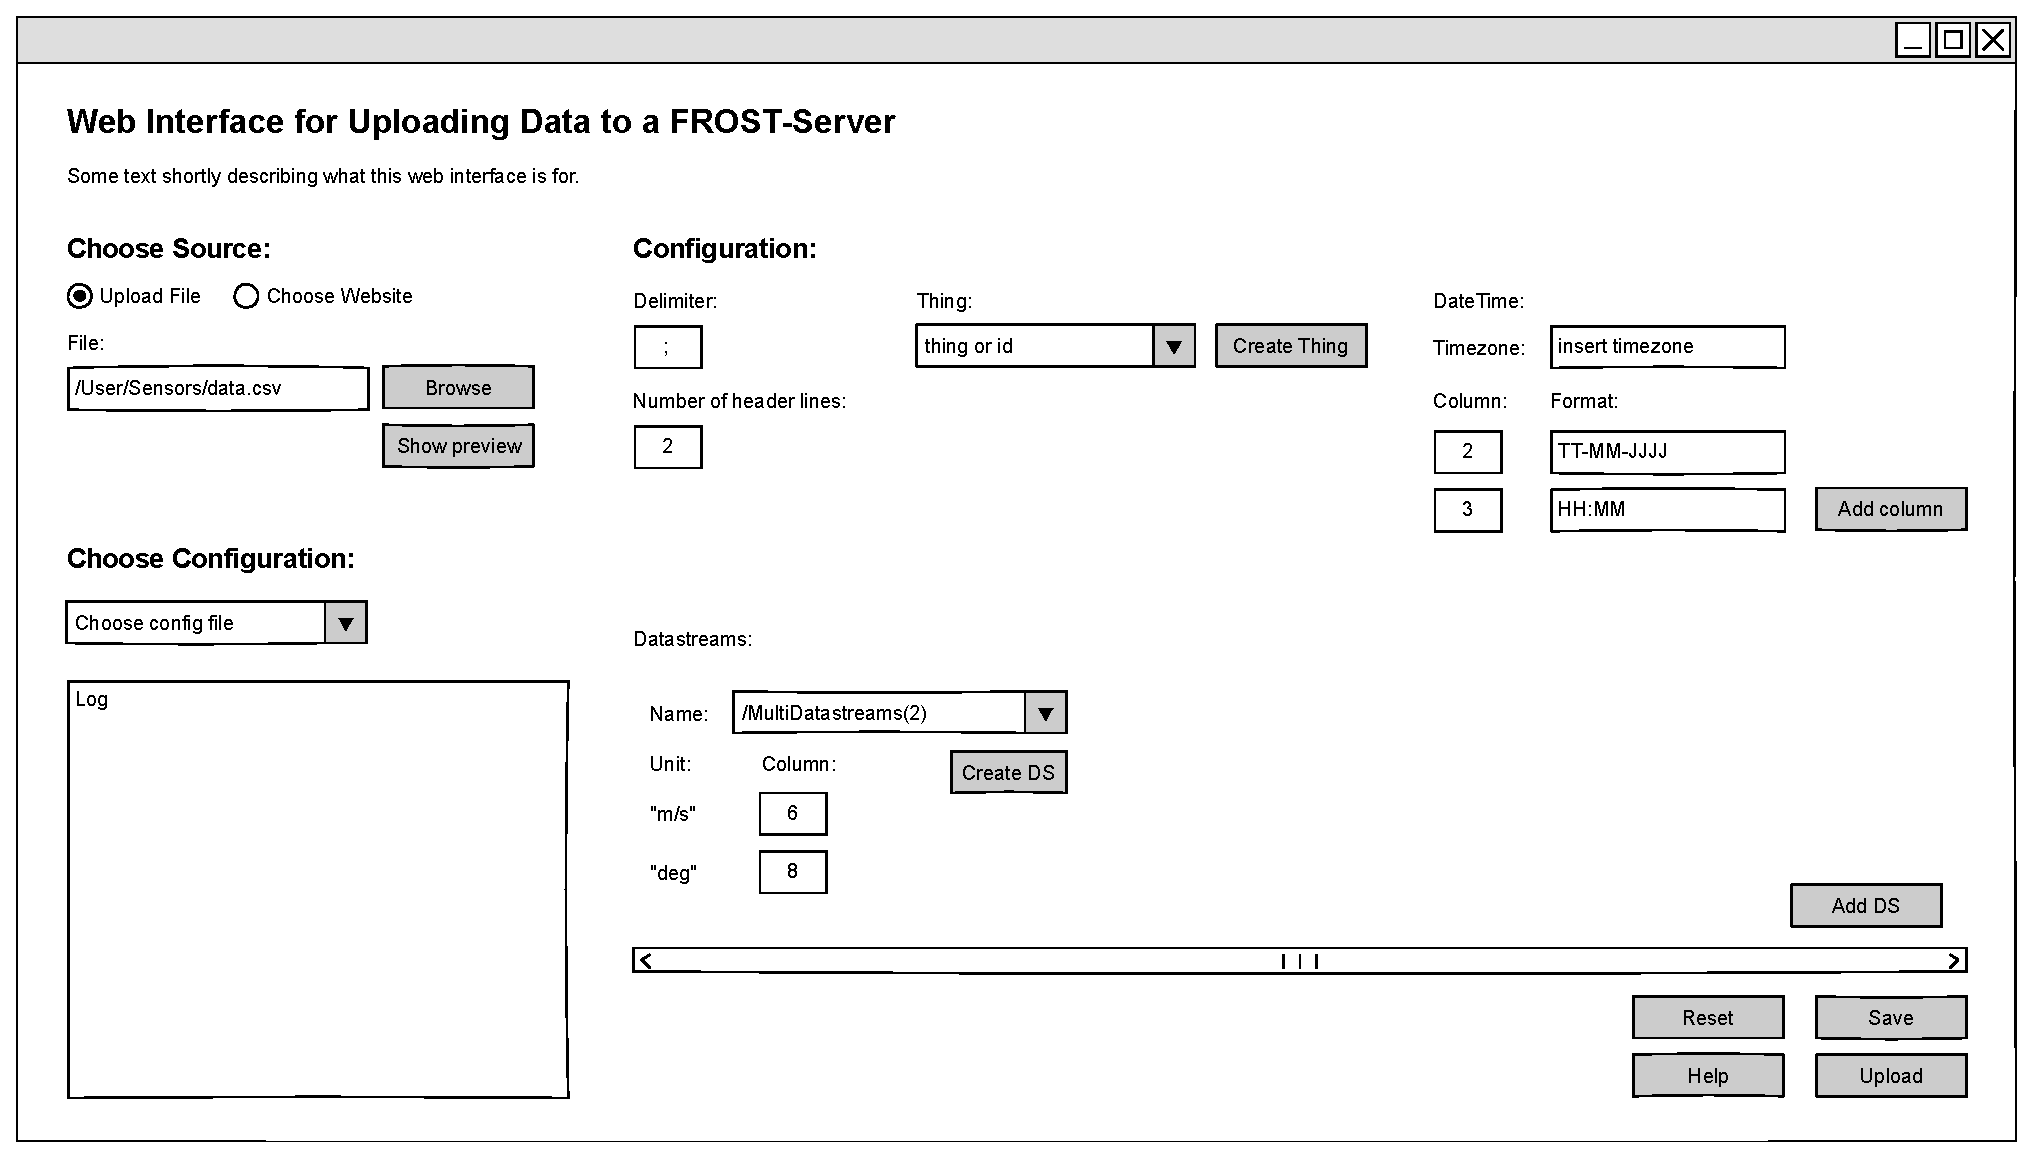
\includegraphics[scale=0.5, angle=90]{images/gui}
\caption{\label{fig:guiMainA}Hauptseite der Weboberfläche}
\end{figure}
\end{textblock*}
	
\end{document}
